\documentclass[norsk, 10pt, twocolumn, a4paper]{revtex4}
\usepackage[T1]{fontenc} %for å bruke æøå
\usepackage[utf8]{inputenc}
\usepackage{amsmath, amsfonts, amssymb, mathrsfs}
\usepackage{graphicx} %for å inkludere grafikk
\usepackage{verbatim} %for å inkludere filer med tegn LaTeX ikke liker
\usepackage{mathpazo}
\usepackage{listings}
\usepackage{color} %red, green, blue, yellow, cyan, magenta, black, white
\definecolor{mygreen}{RGB}{28,172,0} % color values Red, Green, Blue
\definecolor{mylilas}{RGB}{170,55,241}

\bibliographystyle{plain}

\begin{document}

\title{The Ising model and the Metropolis algorithm: \\ Ferromagnetic phase transitions \\ FYS3150 Project 4}
\author{Candidate number: 7 \\ Vilde Flugsrud}
\date{\today}

\begin{abstract}
    \center{\textbf{Abstract}}
    Overall aim: determine the Curie temperature $T_c$ of a system which undergoes a phase transition from ferromagnetic
    to paramagnetic when temperature is raised above a critical temperature, which corresponds to the Curie temperature. We want
    to solve the problem by modeling it with the Ising model and apply Monte Carlo methods through the Metropolis algorithm.

\end{abstract}

\maketitle

\section{Introduction}
-Why relevant. Aims and rationale for the physics case
-What have I done
-Structure of the report

\section{Theory and method}
\subsection{The physics problem}
\subsubsection{How does magnetism arise in the first place?}
Magnetism arises from two sources; electric current and the magnetic moment
induced by the spin of elementary particles, magnetic moment being a measure of the strength of a magnetic source and a
quantity which determines the torque a magnet will experience in an external magnetic field.
This project investigates the latter source. In the context of the magnetization of materials the electrons'
magnetic moments are most important, as the
magnetic moments of the nuclei is much weaker.
The electrons in a material are normally arranged such that their magnetic
moments, orbital and intrinsic, cancel out - they combine into pairs with
opposite intrinsic magnetic moments in accordance with the Pauli exclusion
principle or combine into filled subshels with no net orbital motion.
However, there are solids which may have unpaired electrons or non-filled
subshells. Whether the material produce a magnetic field is then determined
by the direction of the magnetic moments contributed by these electrons.

\subsubsection{Ferromagnetic and paramagnetic}
Ferromagnetic and paramagnetic materials are substances with such unpaired electrons.
In paramagnetic materials the magnetic moments of these tend to point in random directions,
cancelling each other out so that the material is not magnetic (in the
abcense of an external field). The magnetic moments of unpaired electrons in ferromagnetic
materials, on the other hand, have a tendency to allign parallel to one another, as this
leads to lowered energy levels. This effect makes a material magnetic, even in the absence of a
magnetic field.

\subsubsection{Phase transition}
If a ferromagnetic material is raised above a certain temperature, it loses its ferromagnetic
properties. It becomes paramagnetic as the magnetic moments of impaired electrons align
randomly, as a result of the thermal tendency to disorder (increasing entropy) becoming
stronger than the tendency towards lower energy (this drag and pull effect makes up the
thermodynamical potential Helmholtz free energy, described below).

\subsubsection{The Curie temperature}
The temperature at which a ferromagnetic substance experiences this shift is called its
Curie temperature, $T_c$. It is the critical temperature at which the system undergoes a
phase transition from ferromagnetic to paramagnetic. We now have the physics alibi for modeling
this phase transition - if done successfully it allows us to determine $T_c$.

\subsection{The canonical ensemble and the Ising model}
In order to derive the thermodynamical properties of interest, we operate with the canonical ensemble.
An ensemble is a collection of possible states a system might be in, that is it is the probability distribution for the
state of the system. The canonical ensemble describes the possible states available to a system at a fixed temperature
$T$, that is in thermal equilibrium with a heat bath. The system can exchange energy with the heat bath, meaning
the available states may differ in total energy.
This gives a probability for each microstate $i$ dependent on energy, that is $P_i = \frac{1}{Z}e^{-E_i\beta}$.
Here $\beta = \frac{1}{kT}$, $k$ being the Boltzman constant. $e^{-E_i\beta}$ is the Boltzman factor and $Z$ is the
partition function, given below.

We now introduce the Ising model which allows us to model the behaviour of the unpaired electrons'
magnetic moments in the framework of the canonical
ensemble, taking into account the interaction between neighbours.
We model the direction of the
magnetic moments of the electron spins as discrete variables which can be either $+1$ or
$-1$. The spins are arranged in a graph and allowed to interact with its neighbours.
In this project we study the two dimensional Ising model, where the graph corresponds to a
square lattic with $L$ number of spins in each direction.

Given this framework the relevant properties can be computed. We first need the partition function, the sum
of the Boltzman factor of every microstate available to the system, given as

\begin{equation}
    \label{eq:Z}
    Z = \sum\limits_{i=1}^M e^{-E_i\beta} = \sum\limits_E \Omega(E) e^{-E\beta}
\end{equation}
Where $M=2^N = 2^{L\times L}$ is the number of microstates in our two dimensional case. The first expression is a
sum over all microstates. In the second expression we see that microstates with the same
energy will have the same Boltzman factor, making it a sum over all energy levels while multiplying
the Boltzman factor with the corresponding degenerecy.

The energy of each microstate is given by

\begin{equation}
    \label{eq:Ei}
    E_i = -J\sum_{\langle kl \rangle}^N s_k s_l
\end{equation}


The energy expectation value for the canonical ensamble is given as
\begin{equation}
    \label{eq:Eexp}
    \langle E\rangle = -\frac{\delta ln Z}{\delta\beta}
    \langle E\rangle = \sum_{i=1}^M E_i P_i =\frac{1}{Z}\sum_{i=1}^M E_i e^{-E_i\beta}
\end{equation}
using the probability $P_i=\frac{1}{Z} e^{-E_i\beta}$ for a microstate $i$.

The mean magnetization of the system is

\begin{equation}
    \label{eq:Mexp}
    \langle \mathscr{M} \rangle =\sum_{i=1}^M \mathscr{M}_i P_i =\frac{1}{Z}\sum_{i=1}^M \mathscr{M}_i e^{-E_i\beta}
\end{equation}

where the magnetization of one microstate $\mathscr{M}_i$ is given as

\begin{equation}
    \label{eq:Mi}
    \mathscr{M}_i = \sum_{j=1}^N s_j
\end{equation}

that is the sum over all the $N$ spins in one configuration.

As stated earlier, the mechanisms driving the spins to parallel or random alignement is the combination of a strive
towards lower energy and higher entropy,
steered by a system's need to minimize the thermodynamical potential, which for the canonical ensemble is
the Helmholtz free energy $F$:

\begin{equation}
    \label{eq:F}
    F = \langle E \rangle - ST
\end{equation}

$S$ being the entropy.

Phase transitions may be defined as discontinuity in some order derivative of quantities related to the
thermodynamical potential of a given system.
A first order phase transition is marked by a discontinuity in the first order derivative, while a second order
phase transition is marked by a discontinuity in the second order derivative. While the expectation energy is
a first order quantity,
other thermodynamical properties such as the heat capacity $C_v$ are of the second order. This quantity is defined
\begin{align}
    \label{eq:Cv}
    C_v & = - \frac{\delta \langle E \rangle}{\delta\beta} = \frac{\delta^2 lnZ}{\delta\beta^2} \\
        & = \frac{1}{k_BT^2}\sigma_E^2
\end{align}

Where $\sigma_E^2 = \langle E^2 \rangle - \langle E \rangle^2$ is the variance, relating to
the energy fluctuations in the system.

Finally, magnetic susceptibility is given as

\begin{equation}
    \label{eq:chi}
    \chi = \frac{1}{k_BT} \sigma_{\mathscr{M}}^2= \frac{1}{k_BT}(\langle\mathscr{M}^2\rangle - \langle\mathscr{M}\rangle^2)
\end{equation}


\subsubsection{Finite size}
The Ising model has limitations of which the consequences are not neglible. In order for the theory of the canonical ensemble
to be true, we need to operate in the thermodynamical limit, that is the number of spins in each direction $L$
goes to infinity. Thus for every computation we conduct with a fixed value of $L$, we must be aware of the effects of a finite
lattice size.

The finite lattice size require us to handle the end points in the lattice. In this project we do so by periodic
boundary conditions.

\subsection{Analytical calculation $L=2$ lattice}
We first look into the properties of the Ising model analytically, for a small $L=2$ system, 
labeling the spins as $s_1$, $s_2$, $s_3$ and $s_4$ in the following
manner

\begin{align*}
%\begin{pmatrix}
  s_1 \quad s_2 \\
  s_3 \quad s_4 \\
%\end{pmatrix} 
\end{align*}

Thus the energy of a microstate for this lattice size, using equation \ref{eq:Ei}, becomes

\begin{align}
    E_i & = -J(s_1s_2 + s_2s_1 + s_1s_3 + s_3s_1 \\ 
        &+ s_2s_4 + s_4s_2 + s_3s_4 + s_4s_3)
\end{align}

Calculating the energies for the  $M= 2^N = 2^{L\times L}= 16$ microstates we find that there are three possible energies,
that is $-8J$, $0$ and $8J$. The energy $-8J$ is shared by the two microstates with all spins either up or down,
that is $\Omega(-8J)=2$. The energy $0$ is shared by the microstates of three up and one down (four states),
one up and three down (four states), and two up and two down states except the ones where equal spins are on the
diagonals (four states). Thus $\Omega(0) =12$. The energy $8J$ corresponds to the two up and two down states where
equal spins are on the diagonal (two states), giving $\Omega(8J)=2$.

Equation \ref{eq:Z} now gives the $2\times 2$ partition function

\begin{align*}
    Z & = \Omega(-8J)e^{-(-8J)\beta} + \Omega(0)e^{-0\cdot\beta} + \Omega(8J)e^{-8J\beta} \\
      & = 2e^{8J\beta} + 12 + 2e^{-8J\beta} \\
      & = \frac{1}{4}(cosh(8J\beta) + 3)
\end{align*}


From equation \ref{eq:Eexp} we find the mean energy
\begin{align*}
    \langle E\rangle = -8J \frac{sinh(8J\beta)}{3 + cosh(8J\beta)}
\end{align*}

Equations ref{eq:Mexp} and \ref{eq:Mi} gives
\begin{align*}
    \langle \mathscr{M} \rangle = 0 
\end{align*}

Calculating the expectation value of the absolute magnetization one finds
\begin{align*}
    \langle |\mathscr{M}| \rangle = 2\frac{e^{8J\beta} + 2}{cosh(8J\beta) + 3}
\end{align*}

The reason it is of interest to take the absolute value of the magnetization here is the effects of the finite lattice size.
The finite lattice size allows for jumps in the magnetization due to a change of sign which we would not see in the
thermodynamical limit.

From equation \ref{eq:Cv} we calculate the specific heat
\begin{align}
    C_v = \frac{64J^2}{kT^2}(\frac{cosh(8J\beta)}{3+cosh(8J\beta)} - \frac{sinh^2(8J\beta)}{(3+cosh(8J\beta))^2})
\end{align}

While equation \ref{eq:chi} gives the magnetic suceptibility
\begin{align*}
    \chi = \frac{8}{k_BT}\frac{e^{8J\beta}+1}{3+cosh(8J\beta)}
\end{align*}

\subsection{Markov chains, random walk}
The word "ensemble" is also used for a smaller set of possibilities sampled from the full set of possible states. For example, a collection of walkers in a Markov chain Monte Carlo iteration is called an ensemble in some literature.

-It is a Markov Chain

\subsection{Metropolis algorithm}
- The important requirements
- Relation to Markov chains etc
- Relation to Ising Model
-Good: dont need trans. prob. In markov chains gen. not known - for us we dont
need part. func.
To reach this distribution, the Markov process needs to obey two important conditions, that
of ergodicity and detailed balance. These conditions impose constraints on our algorithms for
accepting or rejecting new random states. The Metropolis algorithm discussed here abides
to both these constraints
-Outline the Metropolis algorithm

\subsection{Development of the code. The testing presented in results}

-Abs value of M explain!! - effect on M and chi
-Why we flip 1 and 1 spin
-How we calc the energy changes
-Why LxL times - scale system + get uncorrelated data


-Code for 2x2 case compared to analytic
-Thermalization
the time needed to reach a steady state is longer for temperatures close
to the critical temperature than for temperatures away.
normal to set correlation time $\tau$ equal to thermalization/equilibrium time $t_eq$.
-P(E) (d) OBS: Implement equilibrium thing!! Compare with variance.

-Parallel

\subsection{Phase transition and how to find $T_c$}



-Describe method and algorithm
-How did I implement, my algorithm structure, parts of my code
-Show the reader it reproduces selected benchmarks!!

\section{Results and discussion}
\subsection{2x2, good agreement (table)}
\begin{figure}
    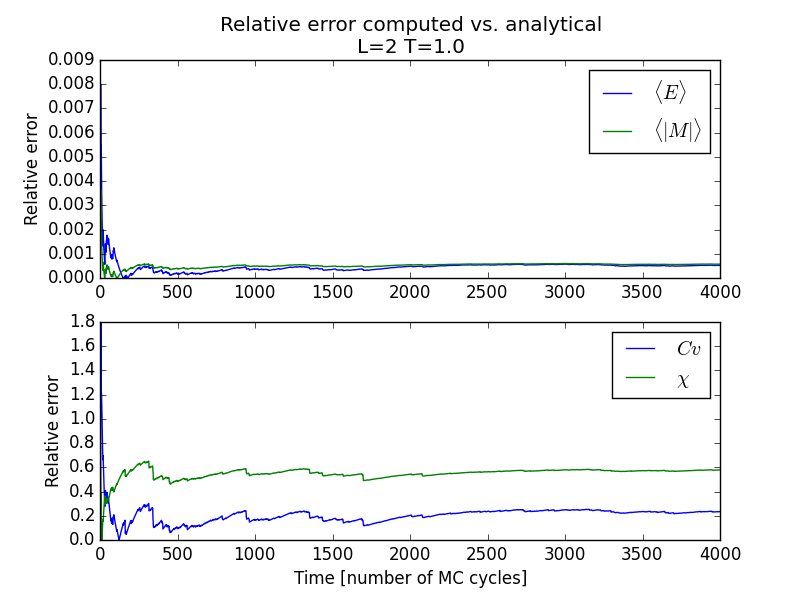
\includegraphics[width=0.9\linewidth]{error.png}
    \caption{
        \label{fig:b1}
        Exp}
\end{figure}
The relative error is plotted in figure \ref{fig:b1}.


\subsection{20x20, when is equilibrium reached? 4 figures + 1 accepted vs cycles fig}
\begin{figure}
    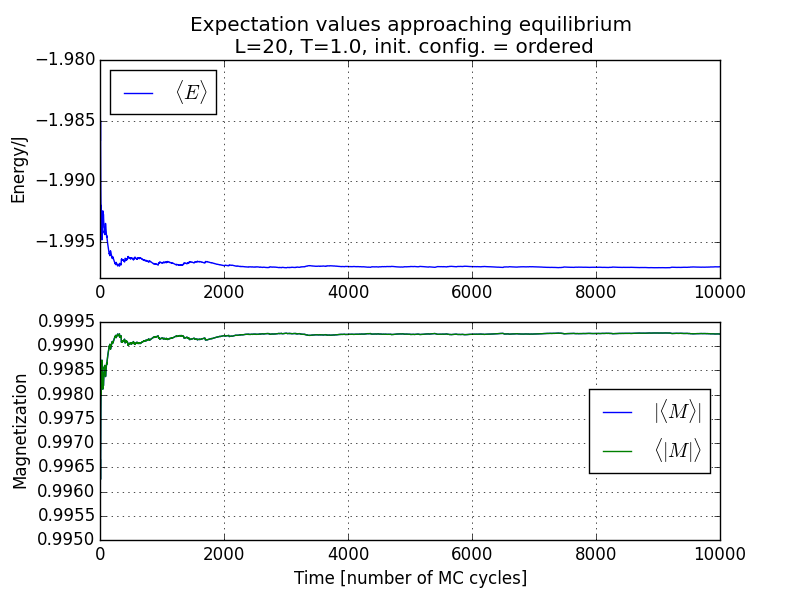
\includegraphics[width=0.9\linewidth]{c_ordered_L20t1mcE4.png}
    \caption{
        \label{fig:c1}
        Exp}
\end{figure}
\begin{figure}
    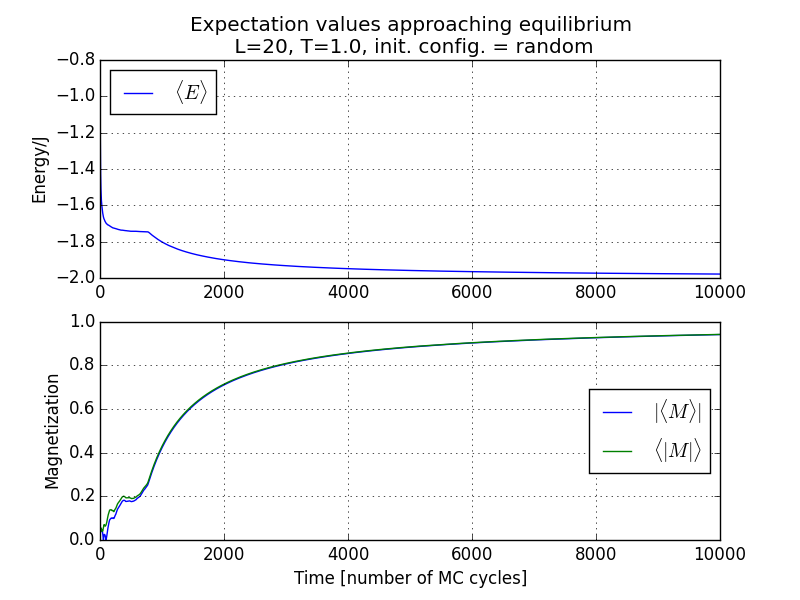
\includegraphics[width=0.9\linewidth]{c_random_L20t1mcE4.png}
    \caption{
        \label{fig:c2}
        Exp}
\end{figure}
\begin{figure}
    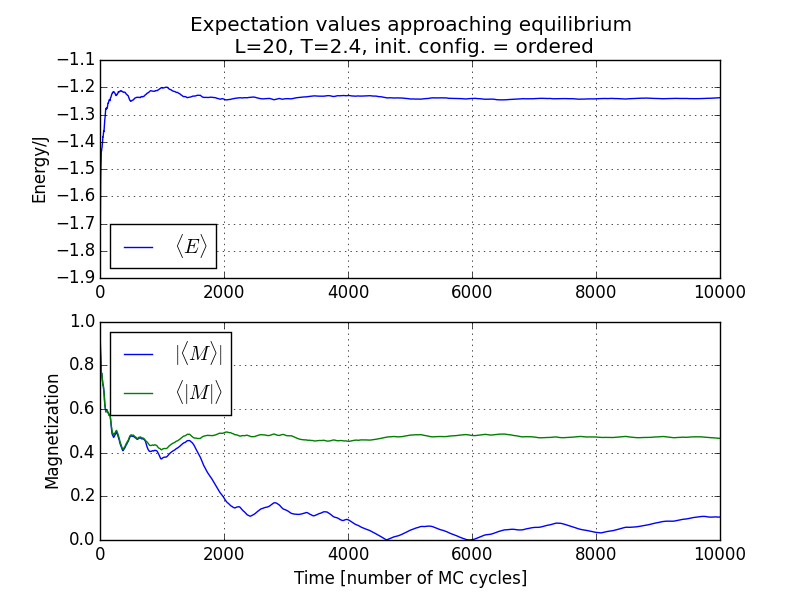
\includegraphics[width=0.9\linewidth]{c_ordered_L20t24mcE4.png}
    \caption{
        \label{fig:c3}
        Exp}
\end{figure}
\begin{figure}
    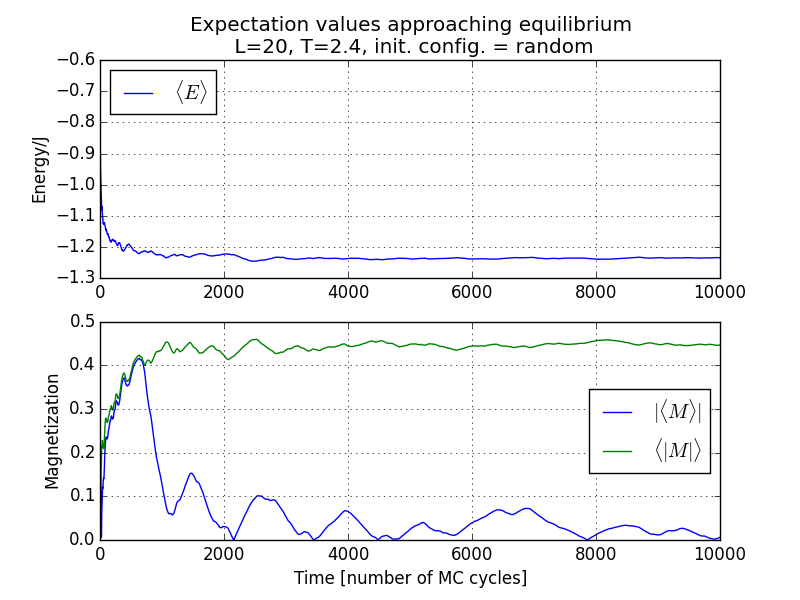
\includegraphics[width=0.9\linewidth]{c_random_L20t24mcE4.png}
    \caption{
        \label{fig:c4}
        Exp}
\end{figure}

\begin{figure}
    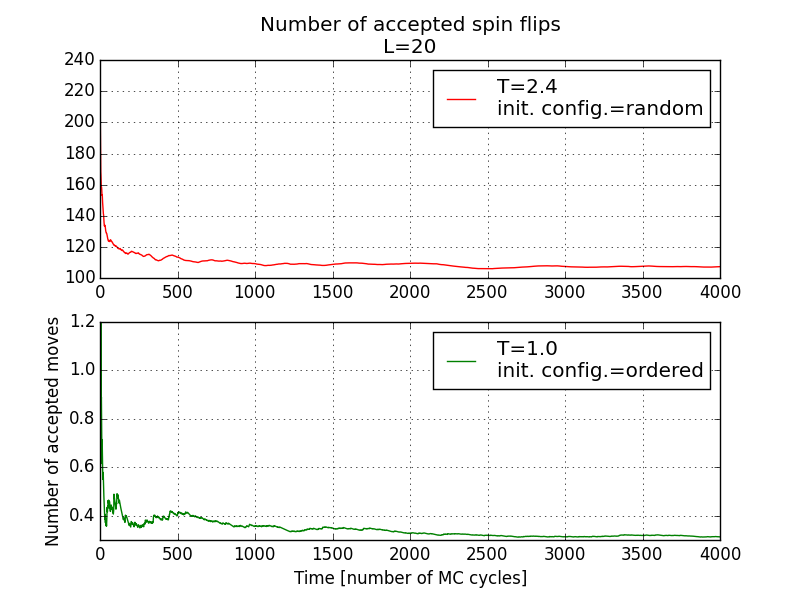
\includegraphics[width=0.9\linewidth]{c_accepted.png}
    \caption{
        \label{fig:c5}
        Exp}
\end{figure}

See figures \ref{fig:c1}, \ref{fig:c2}, \ref{fig:c3} and \ref{fig:c4} for the expectation values plotted against time.
See figure \ref{fig:c5} for the plot of accepted moves against time. 30 percent moves accepted at $T=2.4$.

\subsection{P(E)}
\begin{figure}
    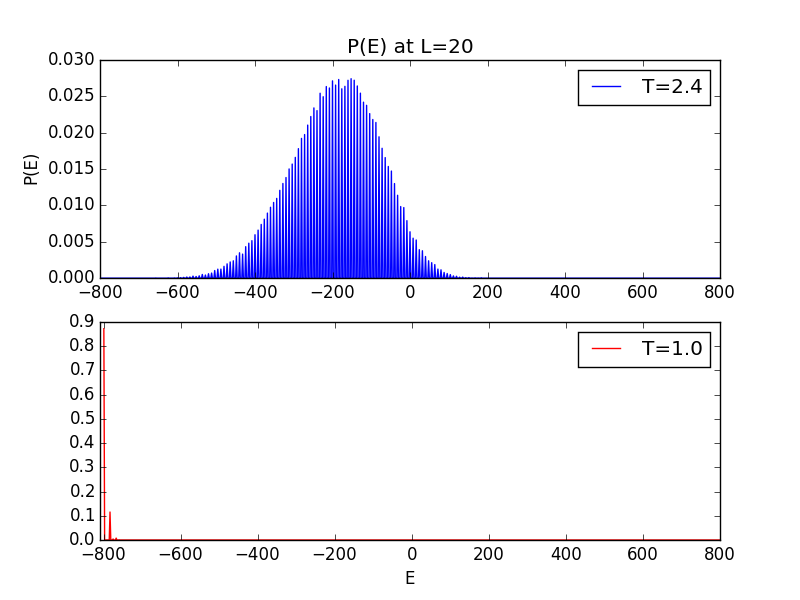
\includegraphics[width=0.9\linewidth]{E_count.png}
    \caption{
        \label{fig:d1}
        Exp}
\end{figure}
See figure \ref{fig:d1}.
Variance: 9.2023609, 3282.654

\subsection{4 plots w/ 4 graphs, parallel}
\begin{figure}
    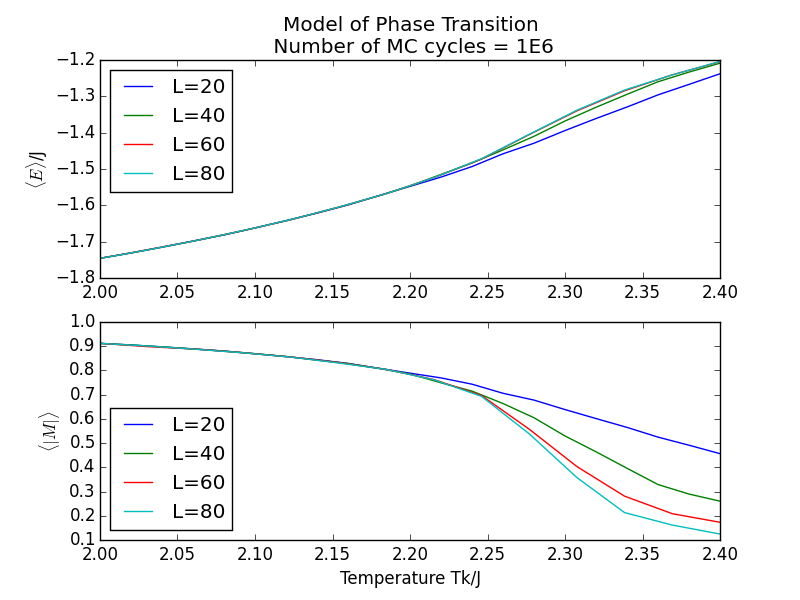
\includegraphics[width=0.9\linewidth]{e1.png}
    \caption{
        \label{fig:e1}
        Exp}
\end{figure}
\begin{figure}
    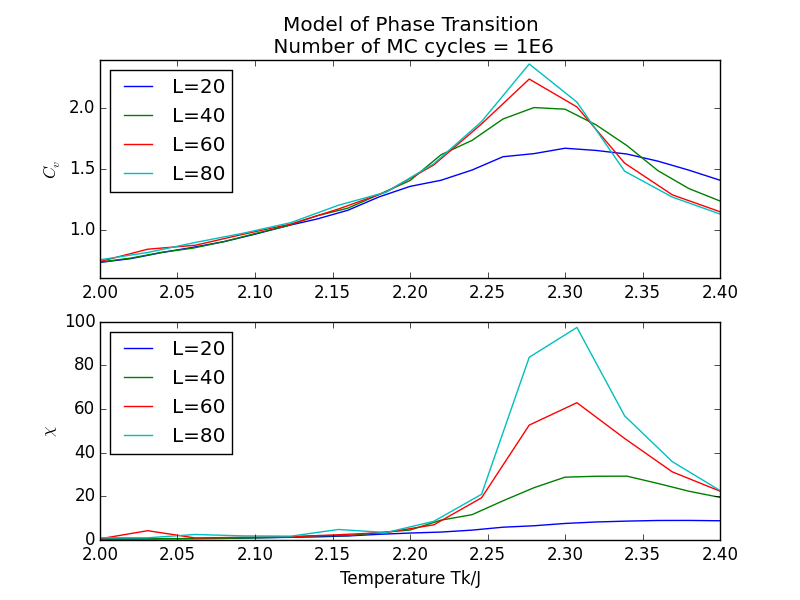
\includegraphics[width=0.9\linewidth]{e2.png}
    \caption{
        \label{fig:e2}
        Exp}
\end{figure}
See figures \ref{fig:e1} and \ref{fig:e2}.


See figure \ref{fig:d1}.

\subsection{Calc of a and Tc}

\section{Conclusion}
Perspectives:
-Autocorrelation func
-Converges(?) sloowly near critical temp because(?) only flip 1 spin at time. Alternative methods


\cite{komp}
\section{Appendix}


\begin{thebibliography}{1}
\bibitem{komp} M. Hjort-Jensen {\em Computational Physics: Lecture Notes}  UiO 2015.

\end{thebibliography}

\end{document}

